% Options for packages loaded elsewhere
\PassOptionsToPackage{unicode}{hyperref}
\PassOptionsToPackage{hyphens}{url}
\documentclass[
]{article}
\usepackage{xcolor}
\usepackage{amsmath,amssymb}
\setcounter{secnumdepth}{-\maxdimen} % remove section numbering
\usepackage{iftex}
\ifPDFTeX
  \usepackage[T1]{fontenc}
  \usepackage[utf8]{inputenc}
  \usepackage{textcomp} % provide euro and other symbols
\else % if luatex or xetex
  \usepackage{unicode-math} % this also loads fontspec
  \defaultfontfeatures{Scale=MatchLowercase}
  \defaultfontfeatures[\rmfamily]{Ligatures=TeX,Scale=1}
\fi
\usepackage{lmodern}
\ifPDFTeX\else
  % xetex/luatex font selection
\fi
% Use upquote if available, for straight quotes in verbatim environments
\IfFileExists{upquote.sty}{\usepackage{upquote}}{}
\IfFileExists{microtype.sty}{% use microtype if available
  \usepackage[]{microtype}
  \UseMicrotypeSet[protrusion]{basicmath} % disable protrusion for tt fonts
}{}
\makeatletter
\@ifundefined{KOMAClassName}{% if non-KOMA class
  \IfFileExists{parskip.sty}{%
    \usepackage{parskip}
  }{% else
    \setlength{\parindent}{0pt}
    \setlength{\parskip}{6pt plus 2pt minus 1pt}}
}{% if KOMA class
  \KOMAoptions{parskip=half}}
\makeatother
\usepackage{longtable,booktabs,array}
\usepackage{calc} % for calculating minipage widths
% Correct order of tables after \paragraph or \subparagraph
\usepackage{etoolbox}
\makeatletter
\patchcmd\longtable{\par}{\if@noskipsec\mbox{}\fi\par}{}{}
\makeatother
% Allow footnotes in longtable head/foot
\IfFileExists{footnotehyper.sty}{\usepackage{footnotehyper}}{\usepackage{footnote}}
\makesavenoteenv{longtable}
\usepackage{graphicx}
\makeatletter
\newsavebox\pandoc@box
\newcommand*\pandocbounded[1]{% scales image to fit in text height/width
  \sbox\pandoc@box{#1}%
  \Gscale@div\@tempa{\textheight}{\dimexpr\ht\pandoc@box+\dp\pandoc@box\relax}%
  \Gscale@div\@tempb{\linewidth}{\wd\pandoc@box}%
  \ifdim\@tempb\p@<\@tempa\p@\let\@tempa\@tempb\fi% select the smaller of both
  \ifdim\@tempa\p@<\p@\scalebox{\@tempa}{\usebox\pandoc@box}%
  \else\usebox{\pandoc@box}%
  \fi%
}
% Set default figure placement to htbp
\def\fps@figure{htbp}
\makeatother
\setlength{\emergencystretch}{3em} % prevent overfull lines
\providecommand{\tightlist}{%
  \setlength{\itemsep}{0pt}\setlength{\parskip}{0pt}}
\usepackage{bookmark}
\IfFileExists{xurl.sty}{\usepackage{xurl}}{} % add URL line breaks if available
\urlstyle{same}
\hypersetup{
  hidelinks,
  pdfcreator={LaTeX via pandoc}}

\author{}
\date{}

\begin{document}

{}

{Livelli di privilegio del modello Cisco}

{1° livello }{user}

{2° livello }{privileged}{\hfill\break
3° livello }{global}

{}

{Per sapere in quale livello mi trovo devo guardare il carattere e il
simbolo.}

{1° livello simbolo `}{\textgreater{}}{'}

{2° livello simbolo `}{\#}{'\\
3° livello simbolo }{`config'}

{}

{Per passare dal livello 1 al livello 2 c'è il comando }{`enable}{'(en)}

{Per passare dal livello 2 al livello 3 c'è il comando `}{configure
terminal}{'(conf t)}

{Per passare dal livello 3 al livello 2 c'è il comando `}{exit}{'(ex)}

{Per passare dal livello 2 al livello 1 c'è il comando `}{disable}{'}

{}

{COMANDI IOS}

{Comandi SHOW: servono per verificare delle cose del mio apparato.}

{Il comando show}{~non }{funziona}{~nell'ultimo livello del Cisco }{solo
nelle prime due}{.}

\begin{itemize}
\tightlist
\item
  {show version}{~(mi mostra la versione e informazioni
  dell\textquotesingle IOS) l'apparato ha principalmente due memoria,
  contiene una NVRam(non volatile) e una DRam(volatile).}
\end{itemize}

\begin{itemize}
\tightlist
\item
  {startup-config modalità con la quale l'apparato parte.}
\item
  {running-config modalità di funzionamento del pc}
\end{itemize}

\begin{itemize}
\tightlist
\item
  {show startup-config}{: mostra il contenuto della nvram ovvero la
  configurazione di avvio}
\item
  {show running-config}{: mostra il contenuto della dram volatile ovvero
  la configurazione di funzionamento. OGNI MODIFICA EFFETTUATA
  UTILIZZANDO I COMANDI IOS VIENE APPLICATA ALLA RUNNING-CONFIG.}
\item
  {copy run start}{: per salvare la configurazione running sulla memoria
  nvram.(ora funziona anche il comando show startup-config)}
\item
  {erase startup-config}{: cancello la configurazione di startup, quindi
  riavviando il dispositivo si cancellerà anche la running config}
\item
  {Show ip interface}{(brief, per le informazioni più importanti): ~}
\item
  {hostname}{: consente di modificare il nome dell'apparato(utile per
  differenziare i diversi apparati tra loro).}
\item
  {Per annullare un comando per tornare indietro bisogna scrivere\\
  }{``no }{configurazione da annullare}{''}{~es. no hostname.}
\item
  {banner motd ``stringa}{''}{: (in modalità config) per dare il
  messaggio di accesso all'apparato.}
\end{itemize}

{}

{}

\subsubsection{\texorpdfstring{{}}{}}\label{h.30j0zll}

\section{\texorpdfstring{{SICUREZZA}}{SICUREZZA}}\label{h.1fob9te}

\begin{itemize}
\tightlist
\item
  {enable password}{~psw faccio in modo che dal livello user a quello
  privilege solo con una psw personalizzata (tuttavia se entro in
  privilege e faccio show running-config vedo la password in chiaro)}
\item
  {enable secret}{~}{psw (una psw diversa): si fa in modalità
  configure(global) e censura la password per accedere al privileged, si
  salva criptata.}
\item
  {line console 0}{: serve per proteggere l\textquotesingle accesso
  tramite il cavo console(proprio per entrare nella modalità user), poi
  si imposta la psw con l\textquotesingle istruzione: }
\end{itemize}

{password}{~}{"psw" e infine digitare il comando }{login}{.}

\begin{itemize}
\tightlist
\item
  {line vty 0 4}{: Per proteggere l'accesso al terminale utilizzando
  telnet o ssh(collegamento tramite cavo UTP) poi si imposta la password
  con il comando password ``psw'' e si digita il comando }{login}{.}
\item
  {service password-encryption}{: cifra tutte le password memorizzate
  nella configurazione running.}
\end{itemize}

{}

{}

\section{\texorpdfstring{{COMANDI SICUREZZA INFORMATICA DI BASSO
LIVELLO}}{COMANDI SICUREZZA INFORMATICA DI BASSO LIVELLO}}\label{h.l8ek275b5ycb}

\begin{itemize}
\tightlist
\item
  {interface fa0/1}{(gig0/1): scelgo una interfaccia(una porta dello
  switch)}
\item
  {switchport mode access}{: }
\item
  {switchport port-security}{:}
\item
  {switchport port-security maximum 1}{: do l'accesso a quella
  porta(fa0/1) solo ad un host(in caso di range sarebbe 1 per ogni
  porta)}
\item
  {switchport port-security mac-address {[}}{mac{]}}{: per fare in modo
  che solo il pc con quel mac possa entrare in quella porta(nel range al
  posto del mac mettiamo ``sticky'' ovvero memorizza i mac in maniera
  automatica)}
\item
  {interface range fa0/2-3}{: proteggo dalla 2 alla 3 di porta dello
  switch}
\item
  {switchport port-security violation }{``(restrict, shutdown(default),
  protect)''}{: mi fa vedere come posso configurare in caso di
  violazione del sistema.}
\end{itemize}

{}

{}

\section{\texorpdfstring{{}}{}}\label{h.8g4h9btxc5h0}

\section{\texorpdfstring{{COMANDI
VLAN}}{COMANDI VLAN}}\label{h.ljszie3jtgtn}

\begin{itemize}
\tightlist
\item
  {vlan {[}num{]}}{~→ }{num \textgreater{} 1 In modalità global }
\item
  {name {[}nome{]}}
\item
  {exit}
\end{itemize}

{interface range fa0/1-5 ~ }

\begin{itemize}
\tightlist
\item
  {switchport access vlan {[}num{]} }{→ }{Assegna le porte alla VLAN del
  numero selezionato.}
\item
  {switchport mode access}{~}{→ }{è facoltativo e permette di non far si
  che la porta o il range di porte non faccia mai trunking}
\item
  {show vlan brief}{~→}{~(In modalità privilege)}{~}{consente di
  verificare l'assegnazione del gruppo di porte alle VLAN create.}
\end{itemize}

{}

\section{\texorpdfstring{{TRUNKING - }{ROUTER ON A STICK (VLAN)
:}}{TRUNKING - ROUTER ON A STICK (VLAN) :}}\label{h.osf1xjmnsjz3}

{router on-a-stick/trunking per utilizzare un solo collegamento per
mettere in comunicazione più vlan}

{Nello switch:}

\begin{enumerate}
\tightlist
\item
  {interface fa0/1 (entriamo nella porta che farà da trunk)}
\item
  {switchport mode trunk ~(Creiamo una dorsale)}
\item
  {switchport trunk allowed vlan add {[}numero vlan{]} (tutto il
  traffico delle vlan passa per quella porta)}
\end{enumerate}

{}

{Nel router:}

\begin{itemize}
\tightlist
\item
  {interface gig0/0.}{{[}nlan{]}}{~-\textgreater{} creazione
  sottointerfaccia per la VLAN}
\item
  {encapsulation dot1Q {[}}{nlan}{{]}}
\item
  {ip address {[}}{indirizzo}{~default gateway{]} {[}subnet mask{]} }
\end{itemize}

{}

{}

\section{\texorpdfstring{{COMANDI INSTRADAMENTO E
ROUTING}}{COMANDI INSTRADAMENTO E ROUTING}}\label{h.mpx6bdf4yfjx}

\begin{itemize}
\tightlist
\item
  {interface fa0/0}{~→ Seleziona l'interfaccia, posso mettere anche vlan
  {[}num{]} al posto della fast se per caso sono su uno switch}
\item
  {ip address {[}IP{]} {[}SUBNET MASK{]}}{~}{→ Assegna l'indirizzo ip e
  la subnet all'interfaccia scelta. Es. ip address 192.168.1.1
  255.255.255.0}
\item
  {ip route {[}IP RETE DEST.{]} {[}SUBNET MASK{]} {[}NEXT HOP{]}}{~→
  Crea una regola di routing.}
\item
  {no shutdown}{~→ Attiva l'interfaccia}
\end{itemize}

{}

{}

\section{\texorpdfstring{{COMANDI
IPV6}}{COMANDI IPV6}}\label{h.sb6sx59gquqo}

\begin{itemize}
\tightlist
\item
  {ipv6 enable}{~→ Abilità l'IPV6 e aggiunge il link-local}
\item
  {ipv6 unicast-routing (in modalità global)}{~→ Abilità l'IPV6}
\item
  {interface GigabitEthernet 0/0}{~→ Entro nell'interfaccia dove devo
  inserire l'ind. ip.}
\item
  {ipv6 address ``indirizzo ipv6''}{~→ Assegna l'indirizzo Global IPV6
  all'interfaccia scelta.}
\item
  {ipv6 address ``indirizzo ipv6'' link-local}{~→ Assegna l'indirizzo
  Link Local IPV6 all'interfaccia scelta.}
\item
  {no shutdown }{→ attivo l'interfaccia.}
\item
  {ipv6 route ``network destination'' ``ip collegamento router''}
\end{itemize}

{}

{Con il comando:}{~ipv6 address address/prefix-length eui-64 }{genero in
maniera automatica un indirizzo ip partendo dal MAC}

{}

{Per assegnare gli indirizzi in maniera automatica:}

{\pandocbounded{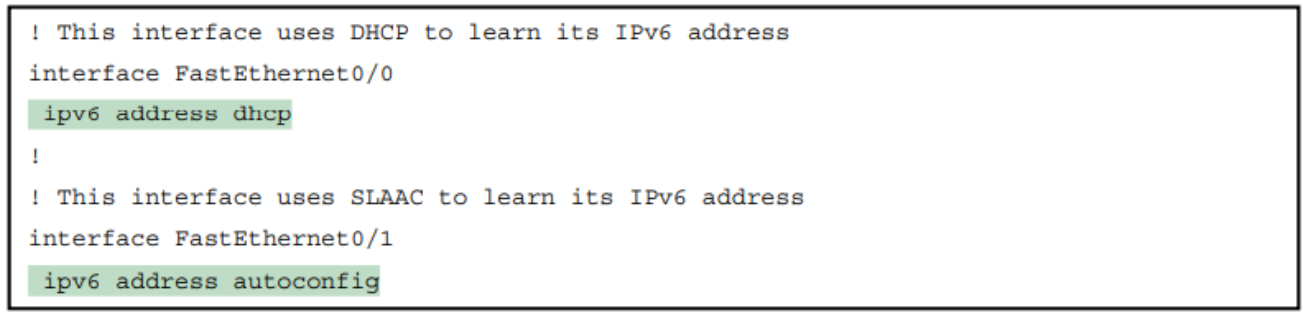
\includegraphics[keepaspectratio]{images/image6.png}}}

{}

{COMANDI CISCO 5°}

{Comandi fatti in quinta:}

{}

\section{\texorpdfstring{{ROUTING
STATIC}}{ROUTING STATIC}}\label{h.ul9owfmafjeq}

{nella sezione }{STATIC}{~del router:}

\begin{itemize}
\tightlist
\item
  {nel Network =\textgreater{} ind. ip dell'altra rete (quella da
  raggiungere);}
\item
  {nel Mask =\textgreater{} subnet mask della rete da raggiungere;}
\item
  {nel Next Hop =\textgreater{} l'ind. del router da cui passare.}
\end{itemize}

{}

{Oppure nella CLI usare il comando: }

{ip route {[}ind IP{]} {[}mask{]} {[}next hop{]} {[}distanza
amministrativa{]}}

{La dist. amm. è facoltativa}

{In base }{all'ind.}{~che metto la rotta può essere:}

\begin{itemize}
\tightlist
\item
  {network}{: fa match con tutta la rete;}
\item
  {predefinita}{: fa match con tutti quelli che non hanno altri match;}
\item
  {host}{: singolo host.}
\end{itemize}

{}

\section{\texorpdfstring{{ROUTING SWITCH LAYER
3}}{ROUTING SWITCH LAYER 3}}\label{h.uvsehtjtly7w}

\begin{itemize}
\tightlist
\item
  {sdm prefer lanbase-routing}
\item
  {reload}
\item
  {ip routing}
\end{itemize}

{}

{creo la vlan, metto l'ind e mask ed eventualmente la accendo}

\begin{itemize}
\tightlist
\item
  {interface }{vlan}{~{[}}{nlan}{{]}}
\item
  {ip address {[}indirizzo{]} {[}mask{]}}
\item
  {no shutdown}
\end{itemize}

{}

\section{\texorpdfstring{{COMANDI
TELNET}}{COMANDI TELNET}}\label{h.pcgz58enxrxl}

{bisogna sempre fare enable secret ma le password}{~}{viaggiano in
chiaro con telnet}

{con SSH invece no. Utile per programmare da lontano lo switch.}

{}

{Comandi base router/switch (in conf t):}

\begin{itemize}
\tightlist
\item
  {line vty {[}range porte es. 0 15{]}}{~ }{nella config verrà segnato
  come line vty 0 4 + line vty 5 15}
\item
  {password {[}``password''{]}}
\item
  {login}
\item
  {exit}
\item
  {enable password/secret {[}``password''{]}}
\end{itemize}

{}

{Per lo switch con VLAN:}

\begin{itemize}
\tightlist
\item
  {interface vlan 1 (vlan di default)}
\item
  {ip address {[}``indirizzo ip della stessa rete ma nuovo''{]}
  {[}mask{]} (come se fosse un host)}
\item
  {no shutdown}
\item
  {line vty {[}range porte{]}}
\item
  {password {[}password{]}}
\item
  {login}
\item
  {exit}
\item
  {ip default-gateway {[}``indirizzo ip''{]}}
\item
  {enable password/secret {[}``password''{]}}{\hfill\break
  }
\end{itemize}

{Nel laptop nel cmd:}

\begin{itemize}
\tightlist
\item
  {telnet {[}IP dello switch messo prima{]}}
\item
  {eventuale password}
\end{itemize}

{}

\section{\texorpdfstring{{COMANDI
SSH}}{COMANDI SSH}}\label{h.cimyzss2yimp}

{Nel router/switch:}

\begin{itemize}
\tightlist
\item
  {ip domain name {[}nome{]}}
\item
  {hostname {[}nome{]}}
\item
  {crypto key generate rsa}
\item
  {1024 o 512 dipende da quanto sicura è la key}
\item
  {username {[}username{]} password {[}password{]}}{~}{distinguiamo chi
  accede, }{creiamo}{~un user+psw per ogni persona che dovrà accedere}
\item
  {ip ssh version {[}numero versione (2){]}}
\item
  {line vty 0 15}
\item
  {transport input ssh}
\item
  {login local}
\end{itemize}

{}

{Con}{~}{show ip ssh }{mostriamo la configurazione}

{}

{Nel cmd:}

\begin{itemize}
\tightlist
\item
  {ssh -L {[}username{]} {[}IP (o il nome messo nell'ip domain name){]}}
\end{itemize}

{\pandocbounded{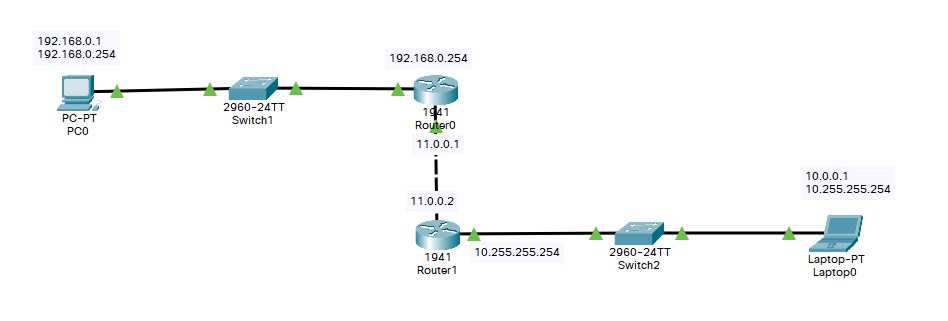
\includegraphics[keepaspectratio]{images/image26.png}}}

{esempio rete con ssh/telnet}

{}

\section{\texorpdfstring{{COMANDI FTP CLIENT E
SERVER}}{COMANDI FTP CLIENT E SERVER}}\label{h.im90xya13xu4}

{Creare tot reti con un server in comune dove andremo a prendere i file;
andare nei }{services}{~nel server, poi nella sezione FTP e aggiungere
un utente.}

{}

{Nel cmd per fare upload sul Server:}

\begin{itemize}
\tightlist
\item
  {ftp {[}indirizzo server{]}}
\item
  {put {[}nome file{]}}
\end{itemize}

{}

{Nel cmd per fare download}{~}

\begin{itemize}
\tightlist
\item
  {ftp {[}indirizzo server{]}}
\item
  {get {[}nome file{]}}
\end{itemize}

{\pandocbounded{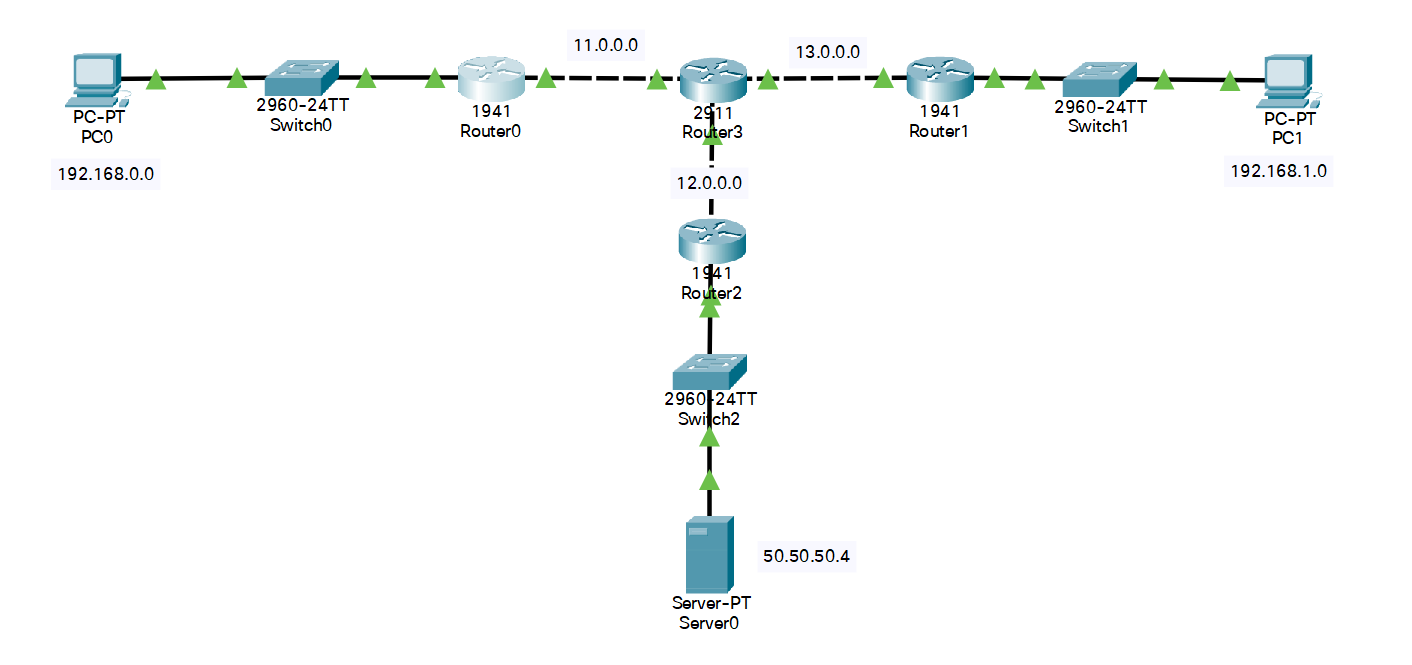
\includegraphics[keepaspectratio]{images/image28.png}}}

{esempio rete con FTP lato server e RIP}

{}

{}

{}

{}

{}

{}

\section{\texorpdfstring{{RIP (Router
popolamento)}}{RIP (Router popolamento)}}\label{h.x9ow7djidmcf}

{Nei vari router in conf t:}

\begin{itemize}
\tightlist
\item
  {router rip}
\item
  {version 2}{~(La versione con Subnet Mask)}
\item
  {network {[}}{ind}{~ip rete1{]}}
\item
  {network {[}}{ind}{~ip rete2{]}}
\end{itemize}

{(Ripetere network tante quante sono le reti da collegare)}

{}

{}

\section{\texorpdfstring{{DHCP}}{DHCP}}\label{h.qf2faznjzg5x}

{In config: DG }

\begin{itemize}
\tightlist
\item
  {ip dhcp pool {[}Lan{]}}
\item
  {network {[}indirizzo di rete{]} {[}SM{]}}
\item
  {default-router {[}ind router{]}}
\item
  {ip dhcp excluded-address {[}indirizzo{]} }{(per non far inserire a
  dhcp alcuni indirizzi)}
\end{itemize}

{}

{Successivamente nel PC possiamo fare }{ip address dhcp}{~per assegnare
uno degli indirizzi nel pool nella macchine}

{}

{}

\section{\texorpdfstring{{COMANDI FIREWALL E
ACL}}{COMANDI FIREWALL E ACL}}\label{h.tig490l5zolq}

{ACL STANDARD SENZA ACCESSO ALLE PORTE}

{In config: DG}

\begin{itemize}
\tightlist
\item
  {access-list {[}numero lista es.1{]} {[}deny/permit{]} {[}indirizzo{]}
  {[}wildcard ovvero il NOT della subnetmask (255.255.255.0 → 0.0.0.255)
  }{dice se vado a isolare una rete o un }{host (0.0.0.0){]}}
\item
  {Esempio1}{~=\textgreater{}}{~}{access list 1 permit any}{~(per
  consentire a tutti di comunicare).}
\item
  {Esempio2 =\textgreater{}}{~}{access list 1 permit 192.168.2.0
  0.0.0.255}{(permette alla LAN con quell'indirizzo di rete di
  comunicare).}
\item
  {Bisogna specificare dove si applicano queste regole: scegliamo
  l'interfaccia di output con: }{interface {[}interfaccia{]}}
\item
  {ip access-group {[}numero lista{]} {[}in/out{]} }{si sceglie }{in
  }{se l'ACL deve essere applicata su un host all'interno della LAN, al
  contrario si sceglie }{out}
\end{itemize}

{}

{ACL ESTESE}

\begin{itemize}
\tightlist
\item
  {access-list {[}numero lista es.101{]} {[}deny/permit{]}
  {[}protocollo{]} host {[}indirizzo mittente{]} host {[}indirizzo
  destinatario{]} eq {[}numero porta lv7{]}}
\item
  {Esempio1 =\textgreater{}}{~}{access-list 101 permit tcp host
  192.168.2.1 host 192.168.1.100 eq 80 }{(il PC con ind. 192.168.2.1 può
  comunicare con il server 192.168.1.100 sulla porta 80)}
\item
  {access-list ~{[}numero lista{]} deny ip any any }{(per negare tutti
  gli altri tipi di traffico)}
\item
  {aggiungere la lista all'interfaccia come nel passo per le acl
  standard}
\end{itemize}

{}

{ACL NAMED}

\begin{itemize}
\tightlist
\item
  {ip }{access-list {[}standard/extended{]} {[}name{]} }{-\textgreater{}
  dopo questo comando tutte le acl fatte saranno già nel gruppo
  {[}name{]}.}
\end{itemize}

{\pandocbounded{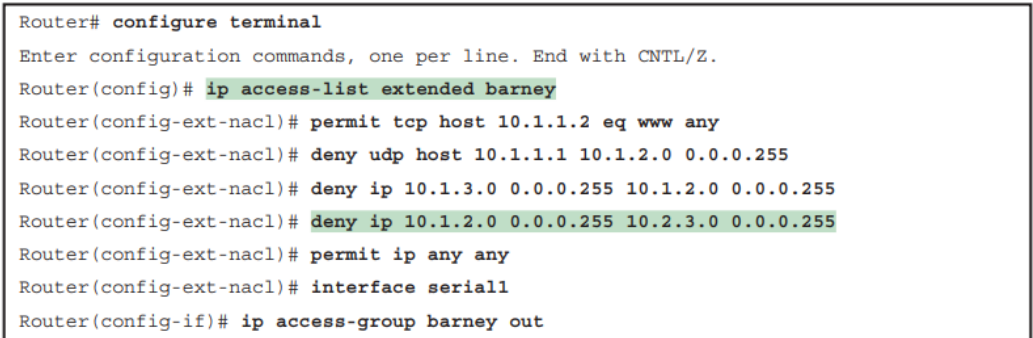
\includegraphics[keepaspectratio]{images/image16.png}}}

{}

{}

\section{\texorpdfstring{{NAT
STATICO}}{NAT STATICO}}\label{h.byiadc8qwbfn}

{In config: DG}

{Sezione inside(da nascondere) da cui arriva il traffico e sezione
outside.}

\begin{itemize}
\tightlist
\item
  {Scegliere l'interfaccia inside}{~(interface {[}interfaccia{]})}
\item
  {ip nat inside}{(nella interfaccia della sezione inside)}
\item
  {exit}
\item
  {Scegliere l'interfaccia outside}{~(interface {[}interfaccia{]})}
\item
  {ip nat outside}{(nella interfaccia della sezione esterna)}
\item
  {ip nat inside source static {[}ip del computer dell'inside{]} {[}ip
  pubblico che assegniamo in maniera statica{]}}{~(sempre nella
  interfaccia dell'outside)}
\item
  {Esempio1 =\textgreater{} }{ip nat inside source static 192,168,1,1
  200.100.50.254}
\item
  {do wr}{~(per applicare la conf. al router, da fare in config)}
\item
  {per vedere il corretto funzionamento fare una request http dal
  browser e usare la simulation}
\end{itemize}

{}

{}

{}

{}

{}

{}

\section{\texorpdfstring{{NAT
DINAMICO}}{NAT DINAMICO}}\label{h.vmvgdbeh4ub}

\begin{itemize}
\tightlist
\item
  {ip nat pool {[}nome pool{]} {[}indirizzo pubblico di partenza pool{]}
  {[}indirizzo pubblico ~di fine pool{]} netmask {[}SM{]}}
\item
  {Esempio1 =\textgreater{} }{ip nat pool nomePool 200.100.50.1
  200.100.50.10 255.255.255.0}
\item
  {access-list 10 permit {[}rete{]} {[}SM al contrario{]}}
\item
  {Esempio2 =\textgreater{} }{access-list 10 permit 192.168.1.0
  0.0.0.255}
\item
  {ip nat inside source list {[}source access list{]} pool
  {[}nomepool{]}}
\item
  {Esempio3}{~=\textgreater{} }{ip nat inside source list 10 pool
  internetworking}
\item
  {Scegliere l'interfaccia inside}{~(interface {[}interfaccia{]})}
\item
  {ip nat inside}{(nella interfaccia della sezione inside)}
\item
  {exit}
\item
  {Scegliere l'interfaccia outside}{~(interface {[}interfaccia{]})}
\item
  {ip nat outside}{(nella interfaccia della sezione esterna)}
\item
  {exit}
\item
  {do wr}{~(per applicare la conf. al router, da fare in config)}
\end{itemize}

{}

\section{\texorpdfstring{{PROTOCOLLI}}{PROTOCOLLI}}\label{h.dllozhjy529h}

\begin{longtable}[]{@{}lll@{}}
\toprule\noalign{}
\endhead
\bottomrule\noalign{}
\endlastfoot
{Nome} & {Porta} & {TCP o UDP} \\
{HTTP/HTTPS} & {80/443} & {TCP} \\
{DHCP} & {68(client)/67(server)} & {UDP} \\
{FTP} & {21(comandi) e 20(dati)} & {TCP} \\
{DNS} & {53} & {UDP/TCP} \\
{SMTP} & {25} & {TCP} \\
{POP3} & {110} & {TCP} \\
\end{longtable}

{}

{}

{COMANDI FATTI ALLA VEM}

\section{\texorpdfstring{{AAA}}{AAA}}\label{h.kpb2xmy5aeem}

{Se in una azienda sono presenti innumerevoli device con utenti
replicati su ognuno, è possibile adottare un server per
l'autenticazione.}

{}

{~``Authentication, authorization, and accounting (AAA) server''}

{}

{Vediamo come configurare uno switch (in config) se è presente un server
AAA RADIUS}{:}

\begin{itemize}
\tightlist
\item
  {aaa new-model}
\item
  {radius-server host {[}IP AAA {]} key {[}key{]}}
\item
  {aaa authentication login default group radius local}{~}{lista di
  metodi di autenticazione (group radius e local)}
\item
  {line }{vty}{~0 5}
\item
  {login authentication default}
\end{itemize}

{}

\section{\texorpdfstring{{Address
table}}{Address table}}\label{h.6tuv10mzbe3n}

{Nello switch:}

{\pandocbounded{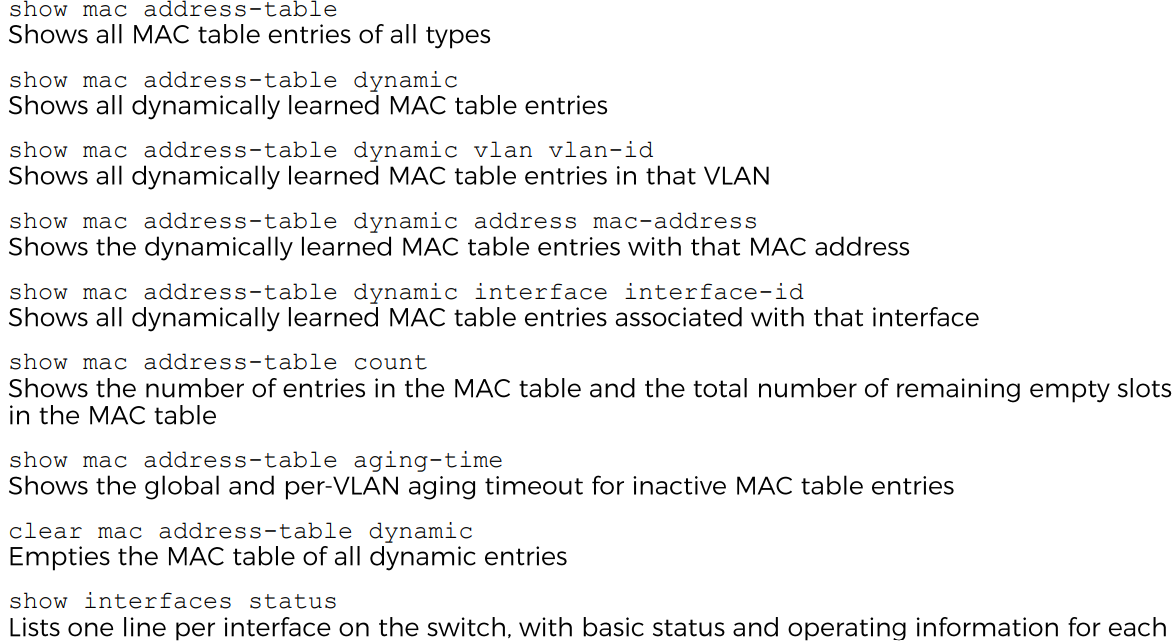
\includegraphics[keepaspectratio]{images/image29.png}}}

{}

{Nel router:}

{\pandocbounded{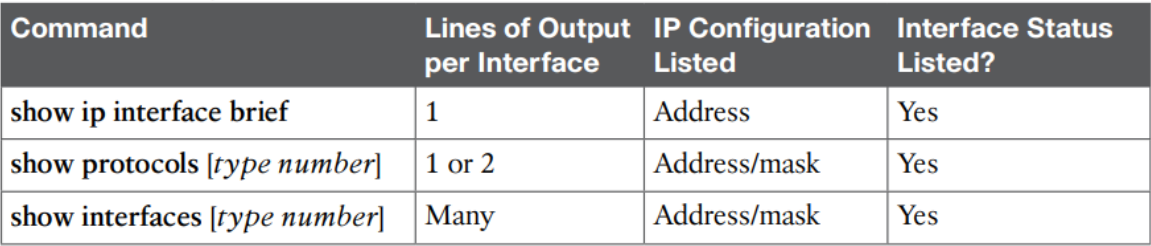
\includegraphics[keepaspectratio]{images/image12.png}}}

{}

\section{\texorpdfstring{{Interfaces
configuration}}{Interfaces configuration}}\label{h.w1tgx7a7s3ev}

{\pandocbounded{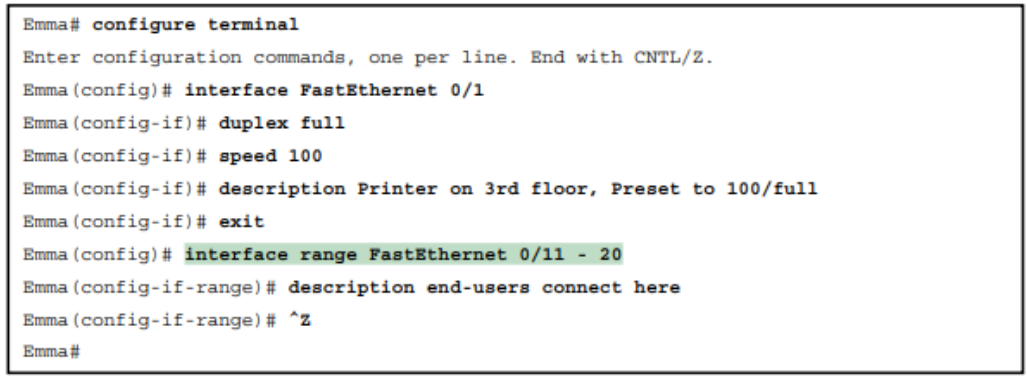
\includegraphics[keepaspectratio]{images/image30.png}}}

{\pandocbounded{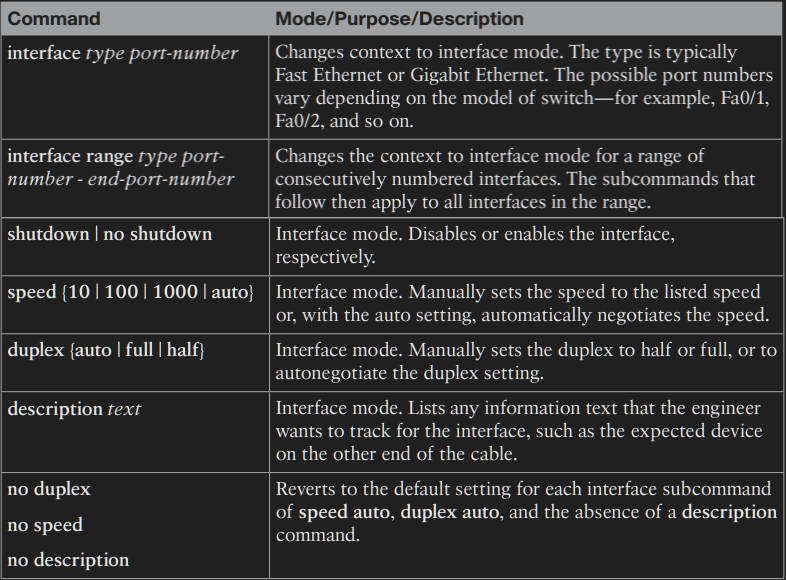
\includegraphics[keepaspectratio]{images/image7.png}}}{\pandocbounded{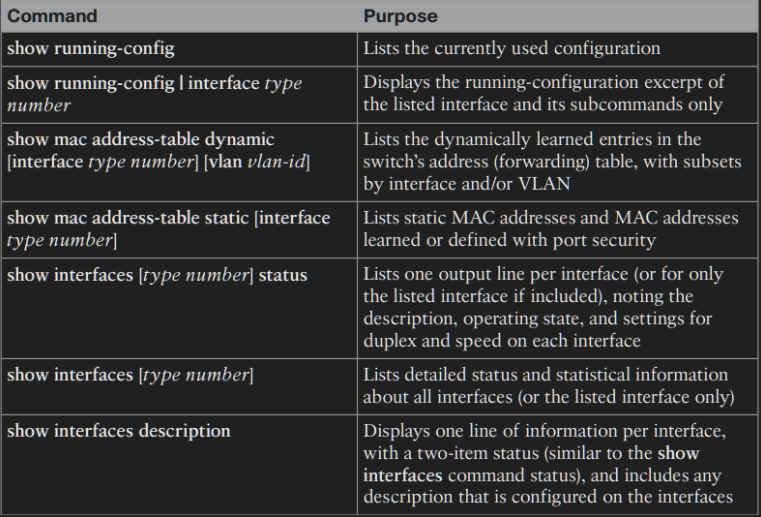
\includegraphics[keepaspectratio]{images/image8.png}}}

{Il comando }{show interfaces}{~restituisce tanti valori nel dettaglio:}

{\pandocbounded{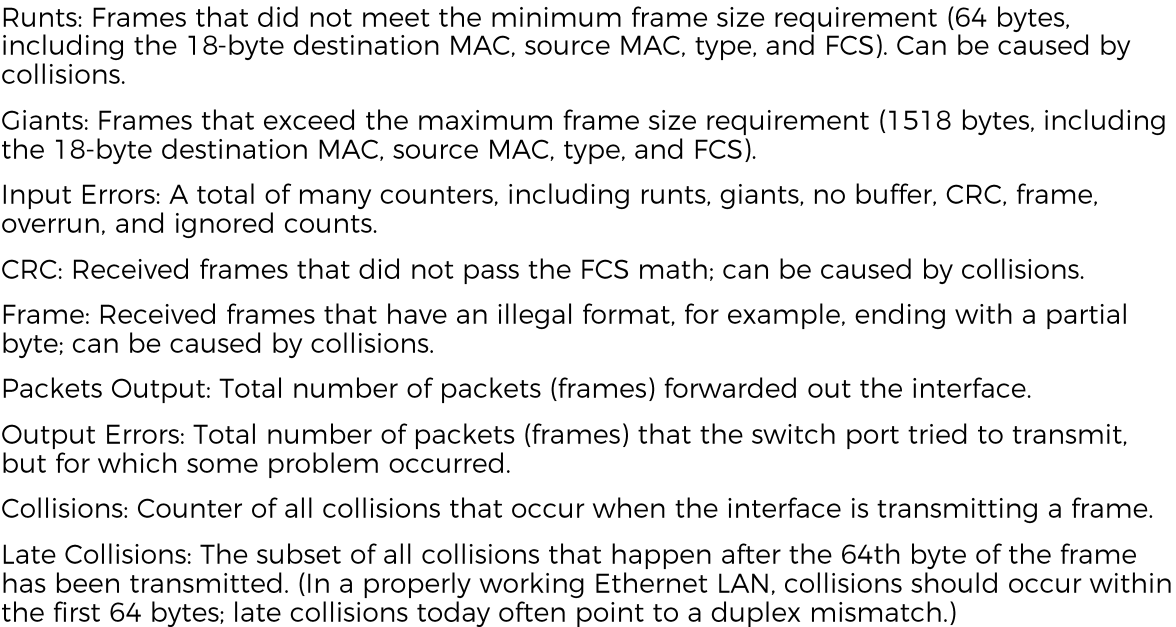
\includegraphics[keepaspectratio]{images/image9.png}}}

{}

\section{\texorpdfstring{{VTP - VLAN Trunking
Protocol}}{VTP - VLAN Trunking Protocol}}\label{h.u9zadesw7sem}

{Serve per propagare in automatico uno VLAN in ogni switch della rete
senza doverle inserire manualmente in ciascuna.}

{}

{Ogni switch può assumere una modalità:}

{\pandocbounded{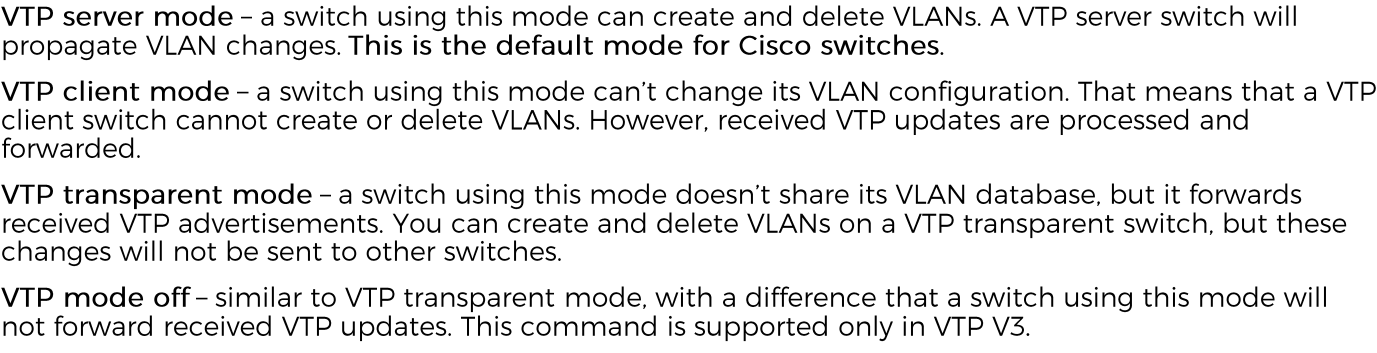
\includegraphics[keepaspectratio]{images/image22.png}}}

{Gli switch server possono coesistere}

{}

{Negli switch server ogni volta che modifichiamo il database delle VLAN
il revision number aumenta e le VLAN vengono propagate in base dallo
switch (anche se non in server mode) con il revision number più grande.}

{Se aggiungo uno switch alla rete con un revision number sbagliato
}{introduco}{~degli errori nelle tabelle degli altri switch, questo
switch sbagliato si chiama }{VTP BOMB}

{}

{\pandocbounded{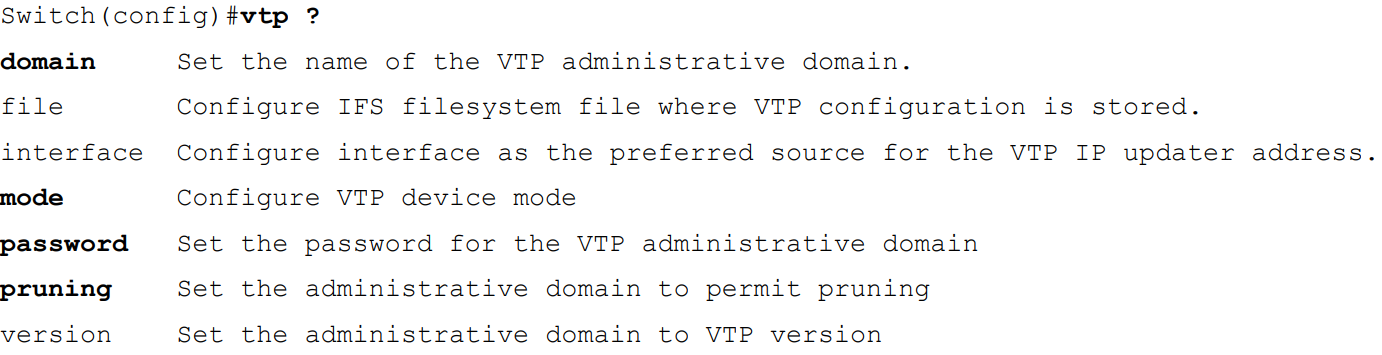
\includegraphics[keepaspectratio]{images/image25.png}}}

{show vtp status}{~-\textgreater{} }{monitoriamo il funzionamento.}

{}

{Il VTP Pruning migliora le prestazioni di rete diminuendo il traffico
non necessario, andando a bloccare frame broadcast verso VLAN che non
hanno interesse in quel messaggio. }

{}

\section{\texorpdfstring{{STP/RSTP}}{STP/RSTP}}\label{h.9dlw0qt8qw69}

{\pandocbounded{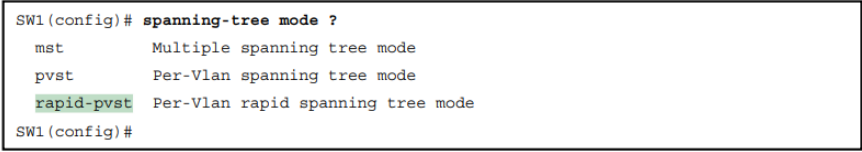
\includegraphics[keepaspectratio]{images/image13.png}}}

{Essendo su apparati Cisco usiamo i loro protocolli che funzionano in
ugual modo a STP/RSTP/MSTP.}

{}

{Si può inserire una priorità ad ogni switch per decidere quale
diventerà lo switch root.}

{\pandocbounded{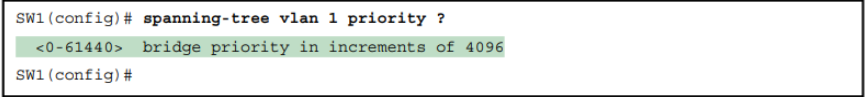
\includegraphics[keepaspectratio]{images/image3.png}}}

{}

{Elenco di comandi:}

{\pandocbounded{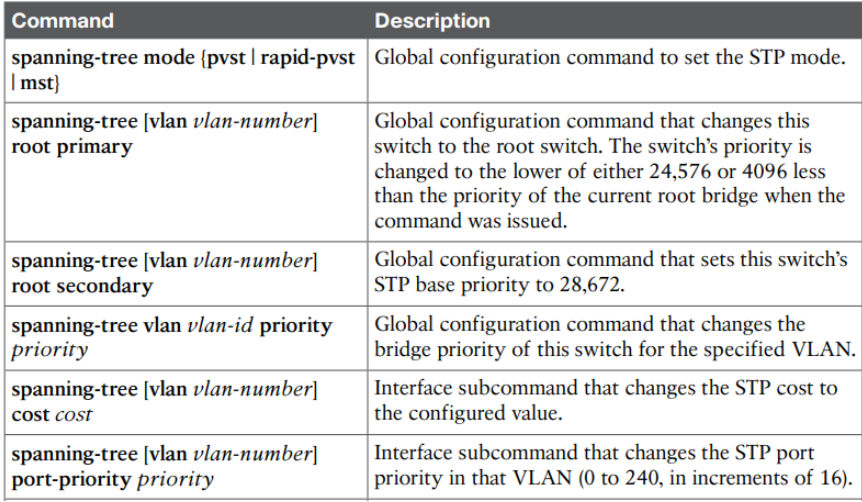
\includegraphics[keepaspectratio]{images/image2.png}}}

\begin{itemize}
\tightlist
\item
  {show spanning-tree}{~=\textgreater{} mostro tutti i dettagli}
\end{itemize}

\section{\texorpdfstring{{PortChannel/EtherChannel}}{PortChannel/EtherChannel}}\label{h.6q0wwybagvu8}

{\pandocbounded{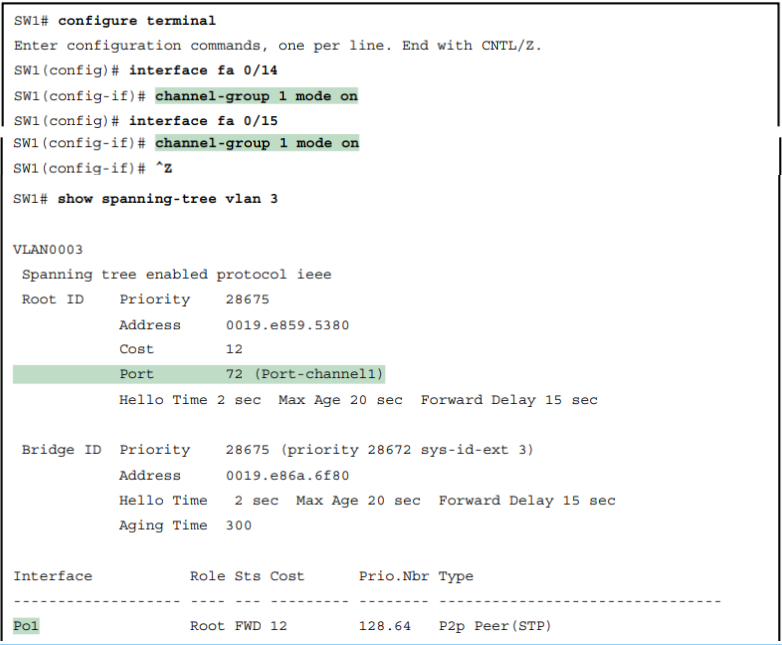
\includegraphics[keepaspectratio]{images/image27.png}}}

{In questo modo STP }{contera}{~i due canali come uno unico e in caso di
guasti non si bloccherà tutto.}

{Per far funzionare il }{PortChannel}{~le porte devono essere uguali,
nel dettaglio:}

{\pandocbounded{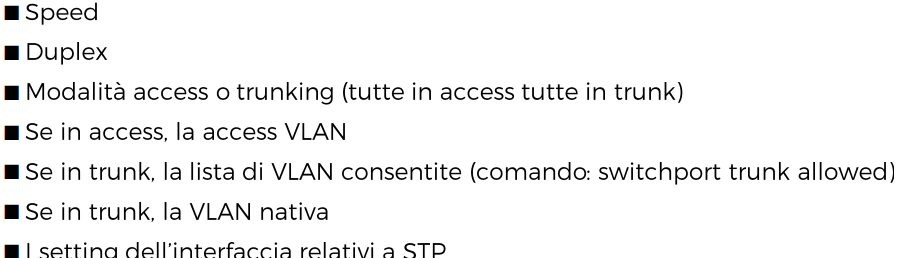
\includegraphics[keepaspectratio]{images/image15.png}}}

{\pandocbounded{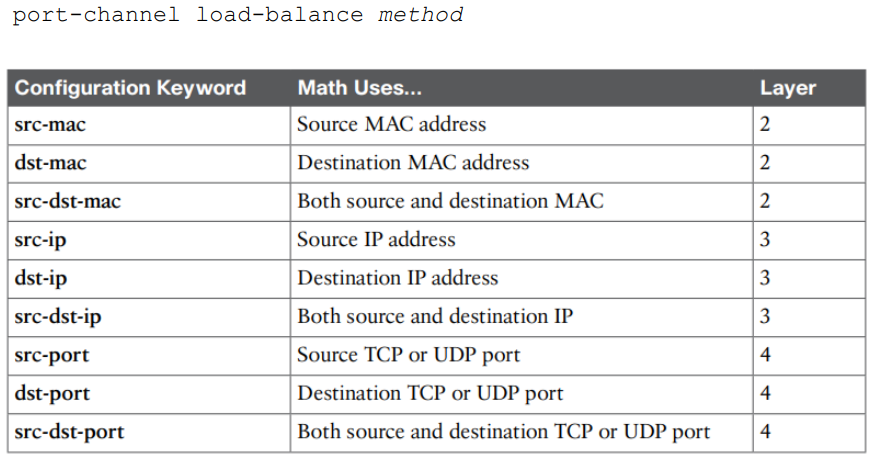
\includegraphics[keepaspectratio]{images/image11.png}}}

{Con questo metodo decidiamo che il traffico verrà bilanciato su tutti i
canali in base a determinati vincoli.}

{}

\section{\texorpdfstring{{Root
Guard}}{Root Guard}}\label{h.my9dwrnsvklt}

{Diciamo che una certa interfaccia eviti i problemi che senza root guard
si }{verificherebbero}{~all\textquotesingle inserimento di un nuovo
switch:}

{\pandocbounded{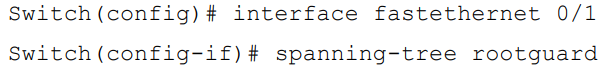
\includegraphics[keepaspectratio]{images/image10.png}}}

{}

\section{\texorpdfstring{{BPDU
Guard}}{BPDU Guard}}\label{h.xs2apqbxqfw3}

{\pandocbounded{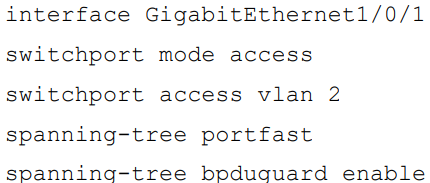
\includegraphics[keepaspectratio]{images/image19.png}}}

{}

\section{\texorpdfstring{{OSPF}}{OSPF}}\label{h.bcljrm2p803h}

\subsection{\texorpdfstring{{Single
Area}}{Single Area}}\label{h.uhlev990b9ok}

{\pandocbounded{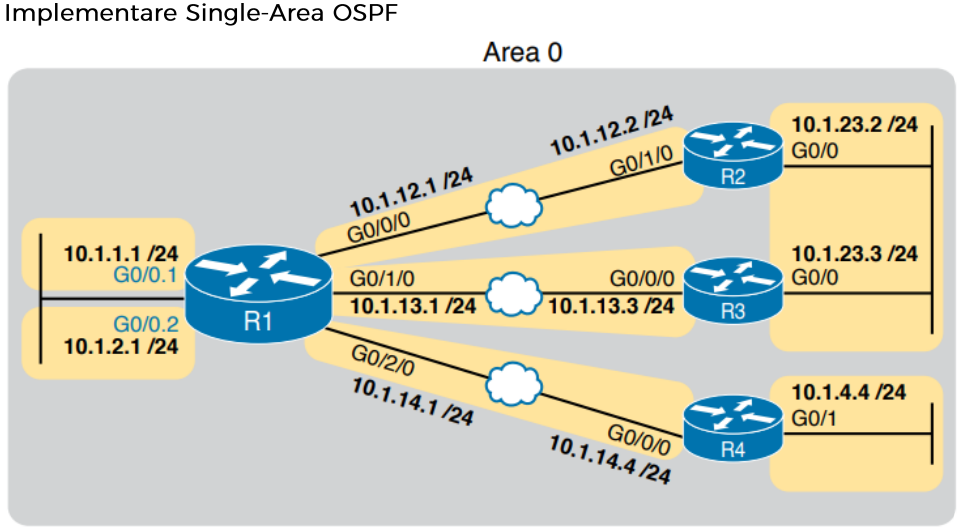
\includegraphics[keepaspectratio]{images/image31.png}}}

{\pandocbounded{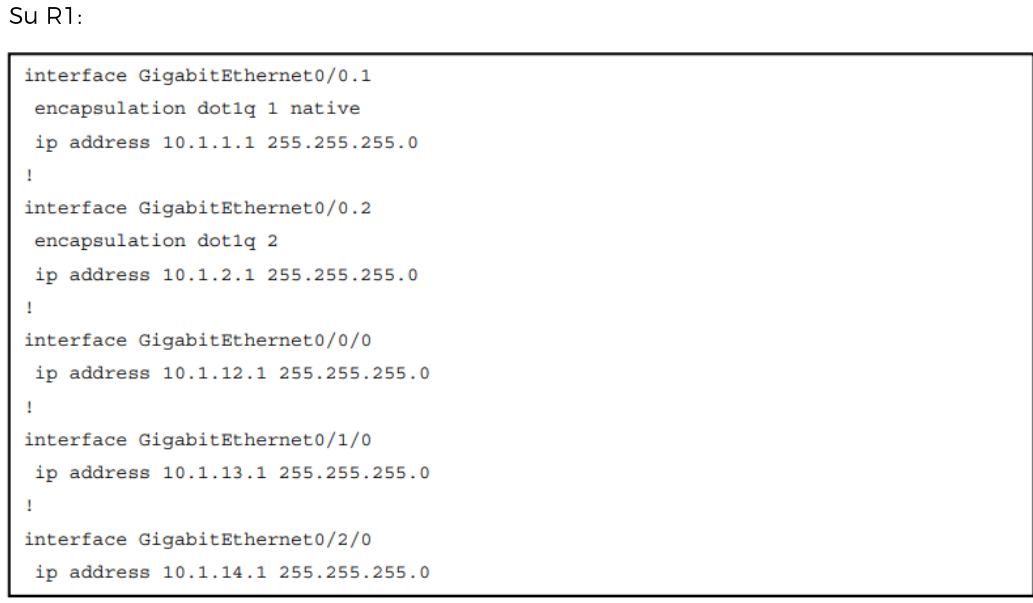
\includegraphics[keepaspectratio]{images/image23.png}}}

{\pandocbounded{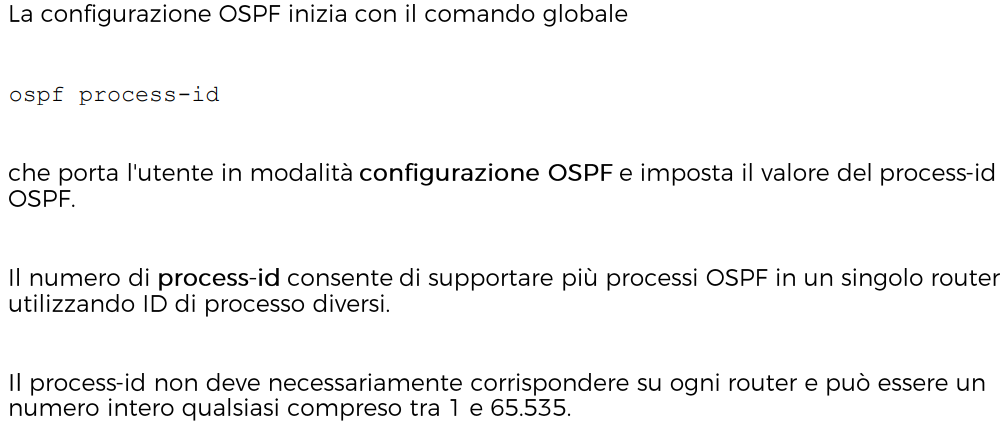
\includegraphics[keepaspectratio]{images/image4.png}}}

{}

{\pandocbounded{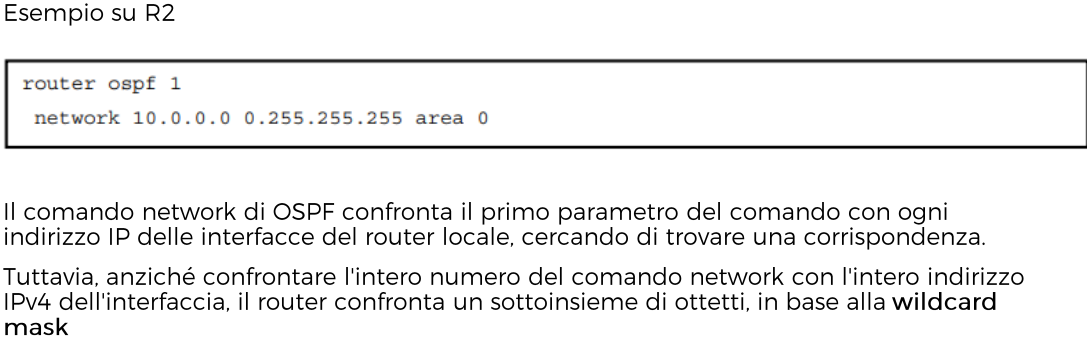
\includegraphics[keepaspectratio]{images/image18.png}}}

{\pandocbounded{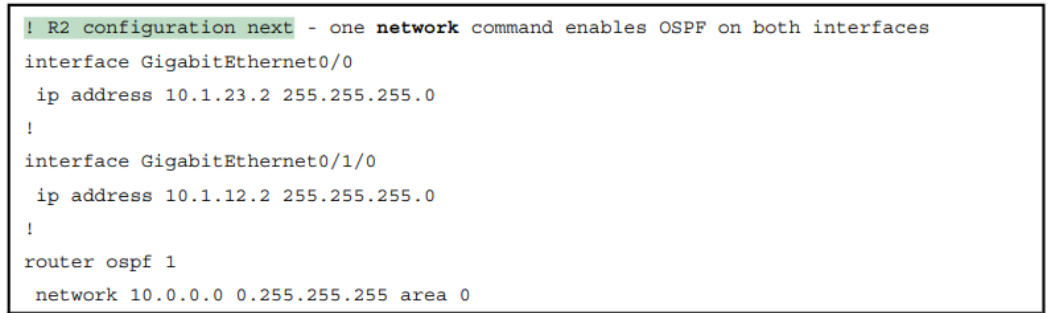
\includegraphics[keepaspectratio]{images/image24.png}}}

{La configurazione degli altri router (R3/4) è simile cambiano gli
indirizzi e le network}

{}

{\pandocbounded{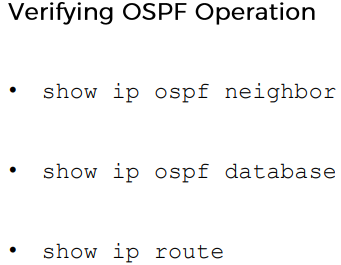
\includegraphics[keepaspectratio]{images/image5.png}}}

{All'invio del primo comando ci uscirà una tabella con una sezione
State, questi sono gli stati disponibili:}

{\pandocbounded{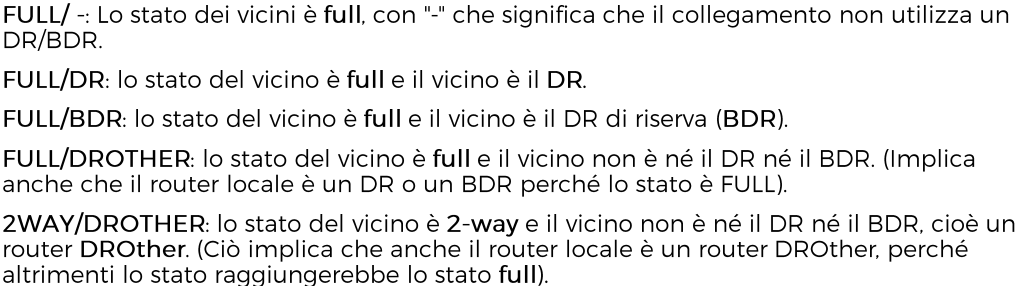
\includegraphics[keepaspectratio]{images/image17.png}}}

\subsection{\texorpdfstring{{Multi
area}}{Multi area}}\label{h.6gs422p47731}

{\pandocbounded{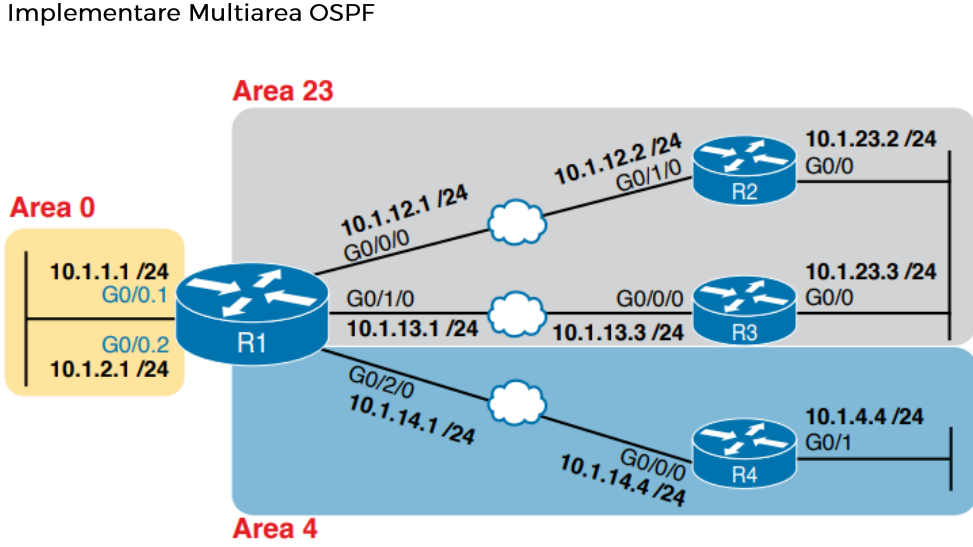
\includegraphics[keepaspectratio]{images/image1.png}}}

{\pandocbounded{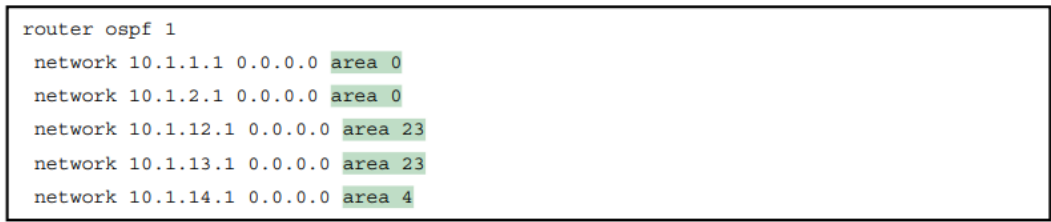
\includegraphics[keepaspectratio]{images/image21.png}}}

{}

{\pandocbounded{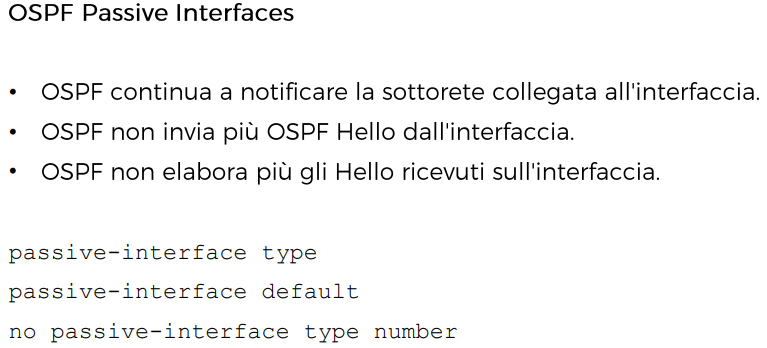
\includegraphics[keepaspectratio]{images/image20.png}}}

{}

{\pandocbounded{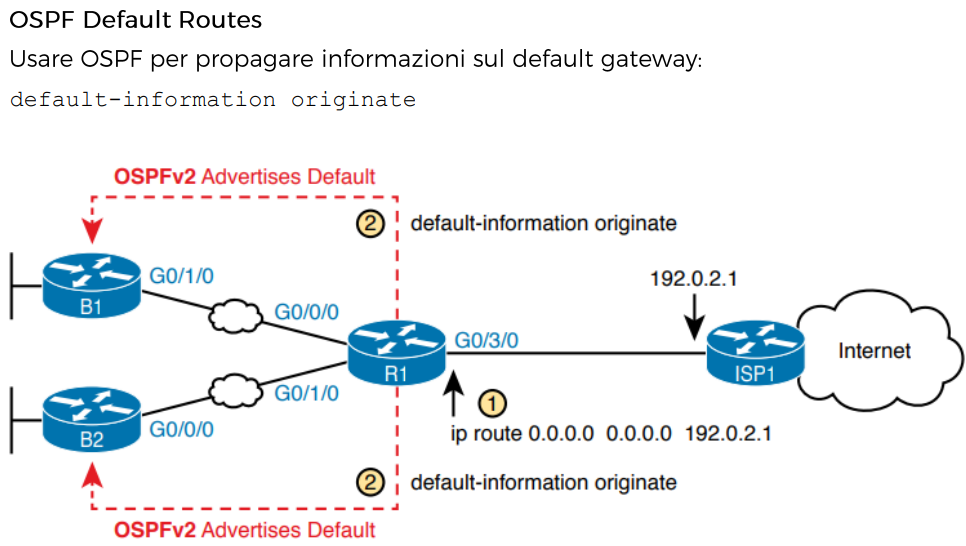
\includegraphics[keepaspectratio]{images/image14.png}}}

{}

{}

\section{\texorpdfstring{{Vari}}{Vari}}\label{h.q6lgnz3v57gd}

\begin{itemize}
\tightlist
\item
  {logging synchronous}{: dice allo switch di aspettare che finiamo di
  scrivere prima di inviare log }
\item
  {history size {[}numero{]}}{: indica quanti comandi la history tiene
  traccia}
\item
  {exec-timeout}{~{[}minuti{]}}{: indica quanto tempo l'utente può
  rimanere inattivo prima di essere kickato}
\end{itemize}

{}

{}

{}

{CONFIGURAZIONE WIRELESS}

{}

{}

\subsubsection{\texorpdfstring{{PRIMO PASSO: config del router
WI-FI}}{PRIMO PASSO: config del router WI-FI}}\label{h.tyjcwt}

{}

\begin{itemize}
\tightlist
\item
  {Scegliamo il router WRT300N;}
\item
  {Clicchiamo sull'apparato e }{selezioniamo GUI}{, andiamo in }{Setup →
  Basic Setup}{~e andiamo in }{Network Setup}{;}
\item
  {Qui scegliamo la configurazione degli indirizzi che vogliamo (l'ip
  del router wireless farà da DG per i dispositivi mobili);}
\item
  {Terminato il setup salviamo con il bottone }{Save Settings}{;}
\item
  {Poi apriamo }{Wireless → ~Basic Wireless Settings}{~e }{impostiamo
  l'SSID}{~con un nome a nostra scelta e salviamo;}
\item
  {Ora apriamo la scheda }{Wireless → Wireless Security }{e impostiamo:}
\end{itemize}

\begin{itemize}
\tightlist
\item
  {la protezione }{WPA2-Enterprise }{con crittografia AES;}
\item
  {l'indirizzo IP del server RADIUS: uno della stessa rete del router;}
\item
  {la Shared Secret.}
\end{itemize}

\begin{itemize}
\tightlist
\item
  {Dopo aver salvato la configurazione router è terminata.}
\end{itemize}

{}

{}

\subsubsection{\texorpdfstring{{SECONDO PASSO: config del server
AAA}}{SECONDO PASSO: config del server AAA}}\label{h.3dy6vkm}

{}

\begin{itemize}
\tightlist
\item
  {Scegliamo un server e nei }{Services }{scegliamo il AAA e impostiamo
  nella }{Network Configuration}{:}
\end{itemize}

\begin{itemize}
\tightlist
\item
  {come Client Name l'SSID della rete wireless;}
\item
  {come Client IP l'ind IP del router wireless;}
\item
  {come Secret la Shared Secret impostata sul router wireless;}
\item
  {come Service Type selezioniamo RADIUS.}
\end{itemize}

{ora con }{ADD}{~aggiungiamo la configurazione creata;}

\begin{itemize}
\tightlist
\item
  {Nella parte sotto (}{User Setup}{) configuriamo le tot. utenze
  previste e clicchiamo }{ADD}{~per }{aggiungerle.}{~}
\end{itemize}

{}

{}

{~}

\subsubsection{\texorpdfstring{{TERZO PASSO: config dei dispositivi
wireless}}{TERZO PASSO: config dei dispositivi wireless}}\label{h.1t3h5sf}

{}

\begin{itemize}
\tightlist
\item
  {Clicchiamo nel dispositivo scelto andiamo in }{Physical }{lo
  spegniamo e cambiamo il modulo Ethernet con uno wireless (}{WMP300N}{)
  e lo riaccendiamo;}
\item
  {In }{Config}{~selezioniamo }{Wireless0}{~e impostiamo:}
\end{itemize}

\begin{itemize}
\tightlist
\item
  {come SSID quello che abbiamo impostato del AAA e nel router;}
\item
  {come metodo di }{Authentication}{~la }{WPA2 }{specificando le
  credenziali;}
\item
  {e come Encryption Type }{AES}{.}
\end{itemize}

\begin{itemize}
\tightlist
\item
  {Questa configurazione è da fare per ogni dispositivo della rete
  wireless.}
\end{itemize}

{}

{}

{}

{}

{}

{}

{MACCHINE VIRTUALI}

{}

{Prerequisiti Macchine Virtuali (Vanno fatti in entrambe le macchine):}

\begin{itemize}
\tightlist
\item
  {Macchina → Impostazioni → Rete}
\item
  {Impostare la rete a ``Rete interna'', lasciare }{intnet}{~come nome.}
\item
  {Configurare gli IP delle due macchine.}
\item
  {Verificare il ping tra le due.}
\end{itemize}

{}

{}

{Procedimento XAMPP}

{La sigla ci dice che l\textquotesingle ambiente che stiamo creando è un
ambiente server con particolari caratteristiche: è un server APACHE
(utilizza MariaDB, PhP e Perl); }

{X: sta ad indicare che è multipiattaforma;}

{A: ci dice apache;}

{M: tipo di database su cui fare le operazioni come mariaDB;}

{P: PHP;}

{P: Perl è un linguaggio;}

{Apache se facciamo start creeremo un server web in locale.}

{se facciamo start in MySQL avremo un database.}

{Infine attiveremo FileZilla e useremo FTP}

{C:\textbackslash XAMPP\textbackslash HTdocs (c'è la pagina web) → al
posto del file index.php creare un file index.html. Questa è la nostra
pagina}

{Per consultare il proprio server nella barra dell'URL di un browser
scrivere 127.0.0.1 oppure localhost/ o anche l'indirizzo IP della
macchina}

{Creare un nuovo index.html si può scorrere anche dentro le cartelle VA
MESSO IL NOME DOPO LA BARRA.}

{}

{Procedimento FileZilla}

{FileZilla: FTP server.}

\begin{itemize}
\tightlist
\item
  {Andiamo su admin; metti password admin dentro XAMPP}
\item
  {Edit setting e mettiamo 0 in tutti timeout i timeout dalle
  impostazioni dell'admin da XAMPP }
\end{itemize}

{per collegarci da un client dobbiamo creare un utente. }

\begin{itemize}
\tightlist
\item
  {edit → ~users → ~add e password}
\item
  {Shared folders → ADD → mettiamo la cartella che vogliamo condividere}
\end{itemize}

{abilita tutto}

\begin{itemize}
\tightlist
\item
  {Avviamo Filezilla client mettiamo host: 127.0.0.1 (Se non usiamo due
  macchine diverse) Nome utente: nome dato alla user e password porta
  lasciarla vuota}
\end{itemize}

{}

\section{\texorpdfstring{{Configurazione di Rete
Windows}}{Configurazione di Rete Windows}}\label{h.2s8eyo1}

{}

\section{\texorpdfstring{{Comandi DNS nel
cmd}}{Comandi DNS nel cmd}}\label{h.17dp8vu}

{ipconfig /displaydns vediamo il contenuto della cache }

{ipconfig /flushdns cancelliamo il contenuto della cache}

{}

\section{\texorpdfstring{{Abilitare connessione desktop remoto
windows}}{Abilitare connessione desktop remoto windows}}\label{h.3rdcrjn}

\begin{itemize}
\tightlist
\item
  {Pannello di controllo}
\item
  {Sistema e sicurezza}
\item
  {Sistema}
\item
  {Impostazioni di connessione remota (a sinistra)}
\item
  {Fare la spunta su ``Consenti connessioni di Assistenza remota al
  computer''}
\item
  {Avanzate:}
\item
  {fare la spunta su ``Consenti il controllo del computer da postazioni
  remote''}
\item
  {Ok}
\item
  {Selezionare ``Consenti connessioni remote al computer''. (In basso)}
\end{itemize}

{}

{}

{}

{SUBNETTING}

{}

\begin{enumerate}
\tightlist
\item
  {Trovare i bit per sottoreti e per host, per i bit della sottorete
  fare 2}{n}{~\textgreater= del numero di sottoreti ( l' n sarà i bit),
  per gli host prendo la sottorete con più host e faccio
  2}{n}{~\textgreater= del numero massimo di host -3 ( l' n sarà i
  bit);}
\item
  {Faccio la somma dei due bit trovati e con la somma trovo la classe
  che devo usare andando a vedere i bit dedicati agli host (Classe A =
  24, Classe B = 16, Classe C = 8), distribuisco eventuali bit restanti
  ( facendo la somma dei bit trovati meno bit degli host di ogni classe
  e andando a scegliere una combinazione);}
\item
  {Prendiamo la combinazione scelta nel passaggio precedente ( Es. 9+7
  con classe B) e decidiamo un indirizzo, preso a caso, ~della classe
  scelta (Es. 172.16.0.0), iniziamo facendo al subnet mask andando a
  prendere quella della classe scelta (Es. classe B =\textgreater{}
  255.255.0.0) e mettiamo a 1 tutti i bit della rete ottenendo così la
  subnet mask (Es. 255.255.}{255}{.}{128}{~=\textgreater{} }{11111111}{1
  }{\textbar{}}{~0000000}{).}
\end{enumerate}

{}

{Per gli indirizzi degli host prendiamo il numero dell'host (Es. 30) e
il numero della sottorete (Es. 4° sottorete) e dividiamo così:}

{172.16.}{1}{.}{158}{~ ~=\textgreater{} ~ }{00000001}{1 }{\textbar{}
}{0011110 }{Nella parte sinistra dove ci sono i bit della rete metto il
numero della sottorete -1 in binario, in quella a destra dove ci sono i
bit destinati agli host metto il numero dell'host in binario.}

{}

{Per il D.G. metto a 1 tutti i bit dedicati agli host tranne l'ultimo
che resta 0}

{~ ~ ~ ~ ~ ~ (Es.1 =\textgreater{} 172.16.}{0}{.}{126
}{=\textgreater{}}{~}{0000000}{0}{~}{\textbar{}}{~}{1111110 ~}{Lo 0
finale nella parte a sinistra perchè 1° sottorete. ~ ~ ~ ~ ~ ~ ~ ~}

{~ ~ ~ ~ ~ ~ ~}{Es.2 =\textgreater{} 172.16.}{0}{.}{254
}{=\textgreater{}}{~}{0000000}{1}{~}{\textbar{}}{~}{1111110 ~}{L' 1
finale nella parte a sinistra perchè 2° sottorete.)}

{}

\end{document}
